\section{Estrutura da Base}

Nesta seção será avaliada a base de recarga do robô, que deve ser fabricada de acordo com as características da estrutura que integra todos os sistemas.

\subsection{Documentação em CAD}
Com a escolha de um carregamento através de indução, problemas com a usinagem dos encaixes entre o robô e seu sistema de carregamentos são solucionados. No sistema que será usado, a tolerância dimensional na fabricação se resume aos pneus do robô tendo um encaixe suave no trilho que serve de guia.

\begin{figure}[H]
	\centering
	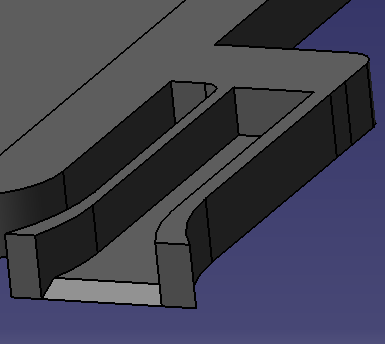
\includegraphics[scale=0.7]{figuras/trilho_base.png}
	\caption{Trilho que será como guia para as rodas.}
	\label{img:trilho_base}
\end{figure}

A ideia é que o robô seja guiado por esses trilhos e fique acomodado em cima da base de recarga, além disso o final do trilho é na exata posição em que o sistema de carregamento que fica na base de recarga e o as baterias do robô estejam em uma posição mais próxima possível, já que a proximidade entre os dois subsistemas é fator muito importante para o tempo de recarga do robô.

\begin{figure}[H]
	\centering
	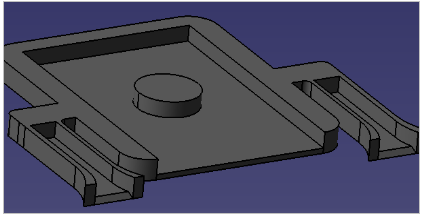
\includegraphics[scale=0.01]{figuras/desenho_base_recarga.png}
	\caption{Desenho da base de recarga.}
	\label{img:desenho_base_recarga}
\end{figure}
